\documentclass[a4paper]{article}
\usepackage[margin=5mm]{geometry}
\usepackage{tikz}
\usetikzlibrary{calc}
\usepackage{xkcdcolors}
\begin{document}
\centering
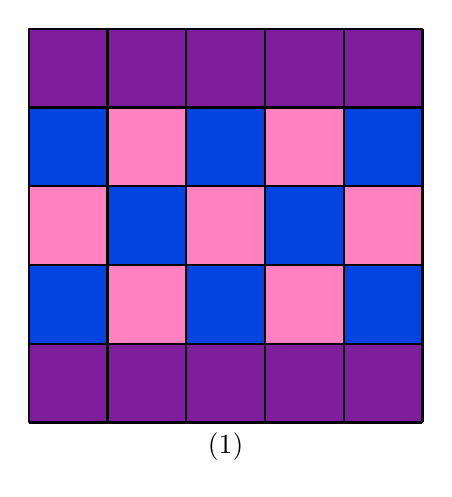
\begin{tikzpicture}
  \filldraw[xkcdPurple] (0,0) rectangle (5,1);
  \filldraw[xkcdPurple] (0,4) rectangle (5,5);
  \filldraw[xkcdPink] (0,1) rectangle (5,4);
  \foreach \x in {1,2,3}{
    \filldraw[xkcdBlue] ({\x-1},\x) rectangle (\x,{\x+1});
    \filldraw[xkcdBlue] ({\x+1},\x) rectangle ({\x+2},{\x+1});
  }
  \filldraw[xkcdBlue] (0,3) rectangle (1,4);
  \filldraw[xkcdBlue] (4,1) rectangle (5,2);
  \draw[thick] (0,0) grid (5,5);
  \node[below] at (2.5,0) {(1)};
\end{tikzpicture}
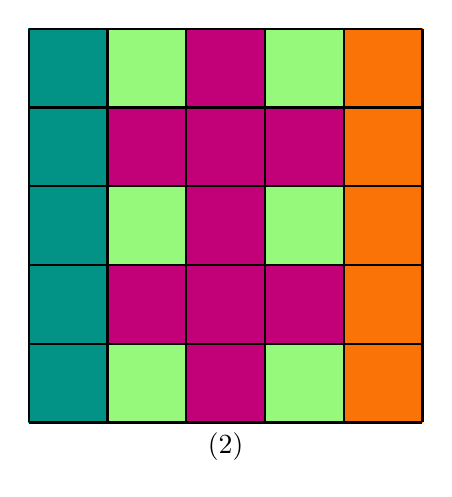
\begin{tikzpicture}[rotate=270]
  \filldraw[xkcdTeal] (0,0) rectangle (5,1);
  \filldraw[xkcdOrange] (0,4) rectangle (5,5);
  \filldraw[xkcdMagenta] (0,1) rectangle (5,4);
  \foreach \x in {1,3}{
    \filldraw[xkcdLightGreen] ({\x-1},\x) rectangle (\x,{\x+1});
    \filldraw[xkcdLightGreen] ({\x+1},\x) rectangle ({\x+2},{\x+1});
  }
  \filldraw[xkcdLightGreen] (0,3) rectangle (1,4);
  \filldraw[xkcdLightGreen] (4,1) rectangle (5,2);
  \draw[thick] (0,0) grid (5,5);
  \node[below] at (5,2.5) {(2)};
\end{tikzpicture}
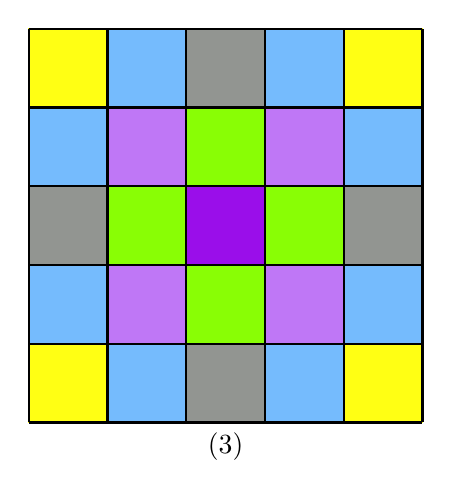
\begin{tikzpicture}
    \filldraw[xkcdSkyBlue] (0,0) rectangle (5,5);
    \filldraw[xkcdLimeGreen] (1,1) rectangle (4,4);
    \foreach \x in {0,4}{
      \foreach \y in {0,4}{
        \filldraw[xkcdYellow] (\x,\y) rectangle ($(\x,\y)+(1,1)$);  
      }
      \filldraw[xkcdGrey] (2,\x) rectangle ($(2,\x)+(1,1)$);  
      \filldraw[xkcdGrey] (\x,2) rectangle ($(\x,2)+(1,1)$);  
    }
        \foreach \x in {1,3}{
      \foreach \y in {1,3}{
        \filldraw[xkcdLightPurple] (\x,\y) rectangle ($(\x,\y)+(1,1)$);  
      }
    }
    \filldraw[xkcdViolet] (2,2) rectangle (3,3);  
  \draw[thick] (0,0) grid (5,5);
  \node[below] at (2.5,0) {(3)};
\end{tikzpicture}

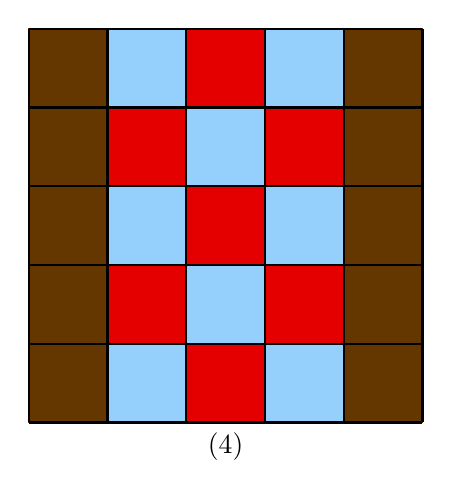
\begin{tikzpicture}[rotate=90]
  \filldraw[xkcdBrown] (0,0) rectangle (5,1);
  \filldraw[xkcdBrown] (0,4) rectangle (5,5);
  \filldraw[xkcdRed] (0,1) rectangle (5,4);
  \foreach \x in {1,2,3}{
    \filldraw[xkcdLightBlue] ({\x-1},\x) rectangle (\x,{\x+1});
    \filldraw[xkcdLightBlue] ({\x+1},\x) rectangle ({\x+2},{\x+1});
  }
  \filldraw[xkcdLightBlue] (0,3) rectangle (1,4);
  \filldraw[xkcdLightBlue] (4,1) rectangle (5,2);
  \draw[thick] (0,0) grid (5,5);
  \node[below] at (0,2.5) {(4)};
\end{tikzpicture}
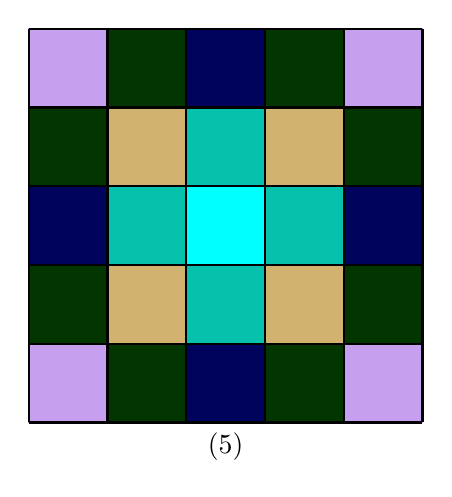
\begin{tikzpicture}
    \filldraw[xkcdDarkGreen] (0,0) rectangle (5,5);
    \filldraw[xkcdTurquoise] (1,1) rectangle (4,4);
    \foreach \x in {0,4}{
      \foreach \y in {0,4}{
        \filldraw[xkcdLavender] (\x,\y) rectangle ($(\x,\y)+(1,1)$);  
      }
      \filldraw[xkcdDarkBlue] (2,\x) rectangle ($(2,\x)+(1,1)$);  
      \filldraw[xkcdDarkBlue] (\x,2) rectangle ($(\x,2)+(1,1)$);  
    }
        \foreach \x in {1,3}{
      \foreach \y in {1,3}{
        \filldraw[xkcdTan] (\x,\y) rectangle ($(\x,\y)+(1,1)$);  
      }
    }
    \filldraw[xkcdCyan] (2,2) rectangle (3,3);  
  \draw[thick] (0,0) grid (5,5);
  \node[below] at (2.5,0) {(5)};
\end{tikzpicture}
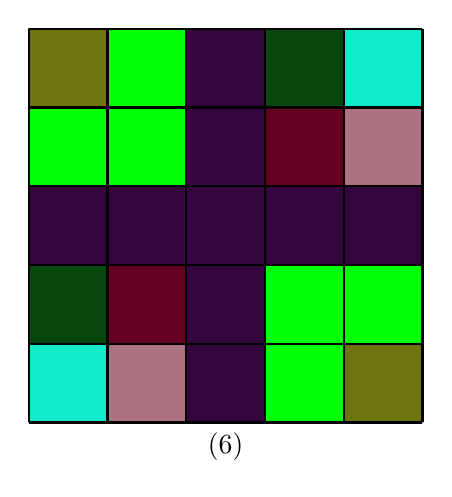
\begin{tikzpicture}
  \filldraw[xkcdAqua] (0,0) rectangle (1,1);  
  \filldraw[xkcdAqua] (4,4) rectangle (5,5);  
  \filldraw[xkcdForestGreen] (0,1) rectangle (1,2);  
  \filldraw[xkcdForestGreen] (3,4) rectangle (4,5);  
  \filldraw[xkcdMauve] (1,0) rectangle (2,1);  
  \filldraw[xkcdMauve] (4,3) rectangle (5,4);
  \filldraw[xkcdMaroon] (1,1) rectangle (4,4);
  \filldraw[xkcdDarkPurple] (2,0) rectangle (3,5);
  \filldraw[xkcdDarkPurple] (0,2) rectangle (5,3);
  \filldraw[xkcdBrightGreen] (3,0) rectangle (5,2);
  \filldraw[xkcdBrightGreen] (0,3) rectangle (2,5);
  \filldraw[xkcdOlive] (0,4) rectangle (1,5);  
  \filldraw[xkcdOlive] (4,0) rectangle (5,1);  
  \draw[thick] (0,0) grid (5,5);
  \node[below] at (2.5,0) {(6)};
\end{tikzpicture}

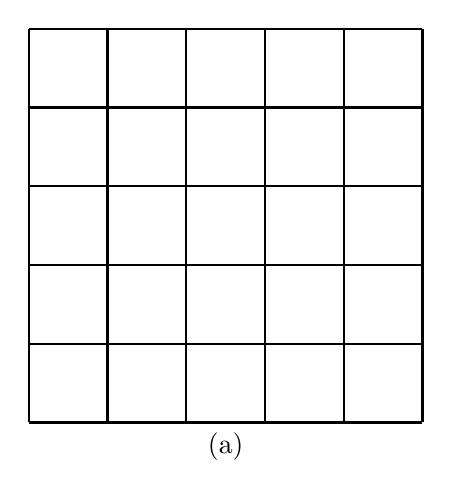
\begin{tikzpicture}
  \draw[thick] (0,0) grid (5,5);
  \node[below] at (2.5,0) {(a)};
\end{tikzpicture}
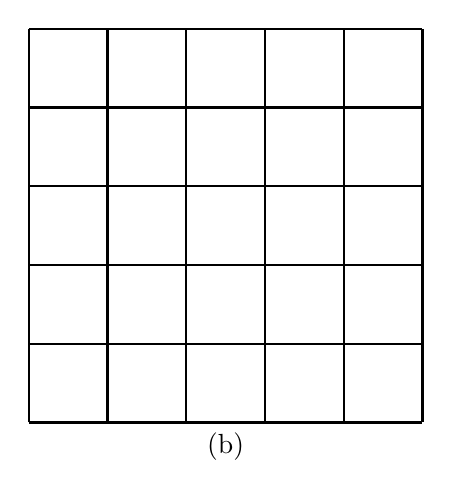
\begin{tikzpicture}
  \draw[thick] (0,0) grid (5,5);
  \node[below] at (2.5,0) {(b)};
\end{tikzpicture}
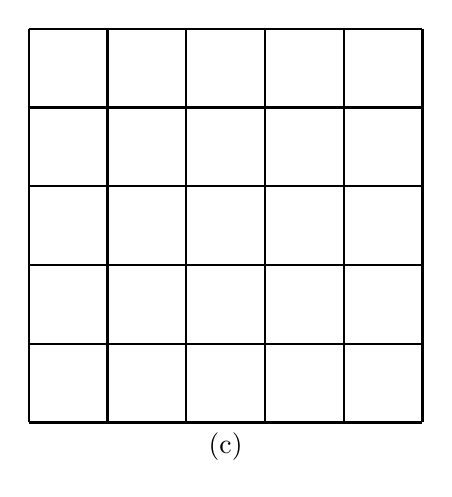
\begin{tikzpicture}
  \draw[thick] (0,0) grid (5,5);
  \node[below] at (2.5,0) {(c)};
\end{tikzpicture}

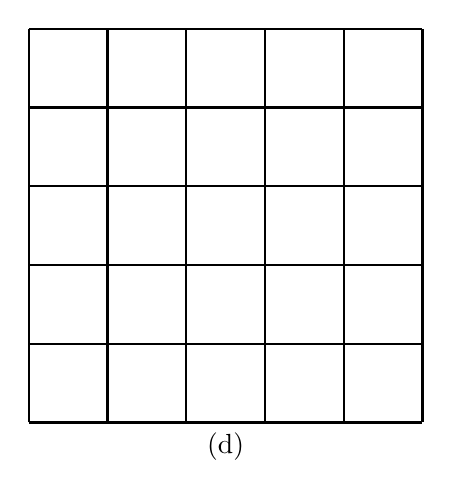
\begin{tikzpicture}
  \draw[thick] (0,0) grid (5,5);
  \node[below] at (2.5,0) {(d)};
\end{tikzpicture}
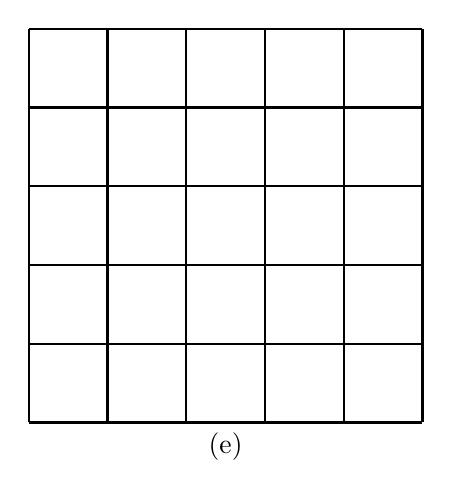
\begin{tikzpicture}
  \draw[thick] (0,0) grid (5,5);
  \node[below] at (2.5,0) {(e)};
\end{tikzpicture}
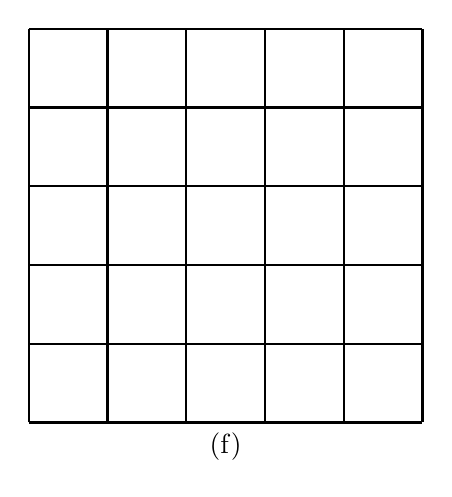
\begin{tikzpicture}
  \draw[thick] (0,0) grid (5,5);
  \node[below] at (2.5,0) {(f)};
\end{tikzpicture}

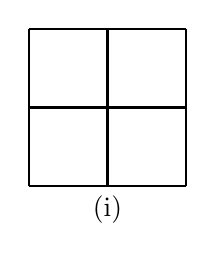
\begin{tikzpicture}
  \draw[thick] (0,0) grid (2,2);
  \node[below] at (1,0) {(i)};
\end{tikzpicture}
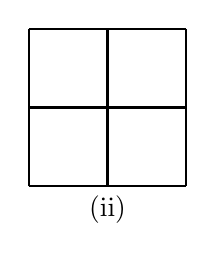
\begin{tikzpicture}
  \draw[thick] (0,0) grid (2,2);
  \node[below] at (1,0) {(ii)};
\end{tikzpicture}
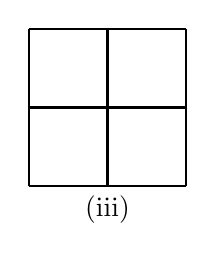
\begin{tikzpicture}
  \draw[thick] (0,0) grid (2,2);
  \node[below] at (1,0) {(iii)};
\end{tikzpicture}
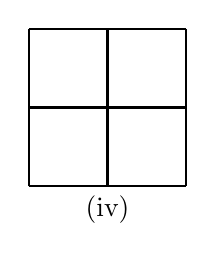
\begin{tikzpicture}
  \draw[thick] (0,0) grid (2,2);
  \node[below] at (1,0) {(iv)};
\end{tikzpicture}
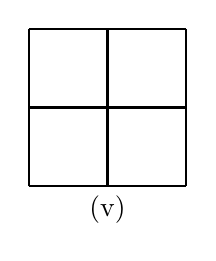
\begin{tikzpicture}
  \draw[thick] (0,0) grid (2,2);
  \node[below] at (1,0) {(v)};
\end{tikzpicture}
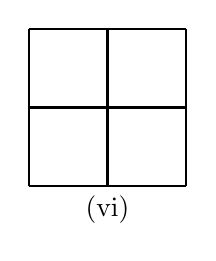
\begin{tikzpicture}
  \draw[thick] (0,0) grid (2,2);
  \node[below] at (1,0) {(vi)};
\end{tikzpicture}
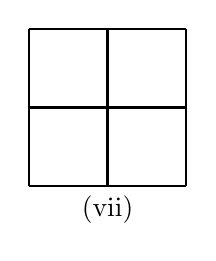
\begin{tikzpicture}
  \draw[thick] (0,0) grid (2,2);
  \node[below] at (1,0) {(vii)};
\end{tikzpicture}
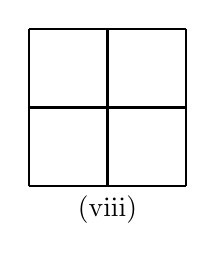
\begin{tikzpicture}
  \draw[thick] (0,0) grid (2,2);
  \node[below] at (1,0) {(viii)};
\end{tikzpicture}

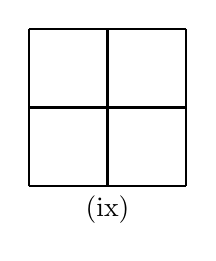
\begin{tikzpicture}
  \draw[thick] (0,0) grid (2,2);
  \node[below] at (1,0) {(ix)};
\end{tikzpicture}
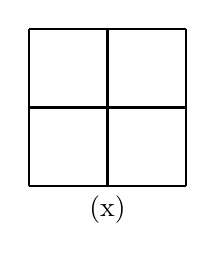
\begin{tikzpicture}
  \draw[thick] (0,0) grid (2,2);
  \node[below] at (1,0) {(x)};
\end{tikzpicture}
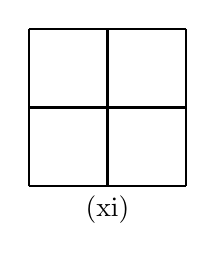
\begin{tikzpicture}
  \draw[thick] (0,0) grid (2,2);
  \node[below] at (1,0) {(xi)};
\end{tikzpicture}
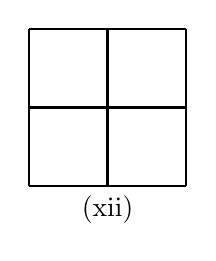
\begin{tikzpicture}
  \draw[thick] (0,0) grid (2,2);
  \node[below] at (1,0) {(xii)};
\end{tikzpicture}
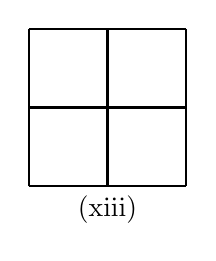
\begin{tikzpicture}
  \draw[thick] (0,0) grid (2,2);
  \node[below] at (1,0) {(xiii)};
\end{tikzpicture}
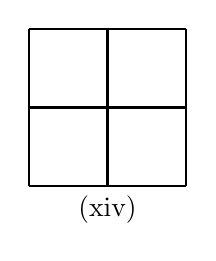
\begin{tikzpicture}
  \draw[thick] (0,0) grid (2,2);
  \node[below] at (1,0) {(xiv)};
\end{tikzpicture}
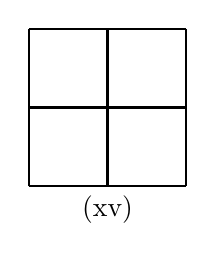
\begin{tikzpicture}
  \draw[thick] (0,0) grid (2,2);
  \node[below] at (1,0) {(xv)};
\end{tikzpicture}
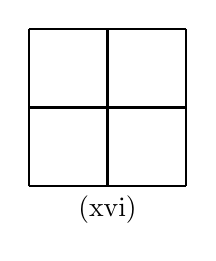
\begin{tikzpicture}
  \draw[thick] (0,0) grid (2,2);
  \node[below] at (1,0) {(xvi)};
\end{tikzpicture}
\end{document}